\documentclass{article}
\usepackage[utf8]{inputenc}
\usepackage{enumitem}
\usepackage{graphicx}

\title{440 Final Project}
\author{Xiaowei Zhang, 204007085 \\ Xinyuan Chen, 197001668}
\date{December 2021}

\begin{document}
\maketitle

\section*{Feature}
For this project, we use the feature extraction by UCB.\\
Digit: Returns a set of pixel features indicating whether each pixel in the provided datum is white (0) or gray/black (1).\\
Face: Returns a set of pixel features indicating whether each pixel in the provided datum is an edge (1) or no edge (0).

\section*{Perceptron}
We initialize the weight to be 0, and then update them later. We stop running when it reaches the max iterations. We have a list to keep the weights for each label and pick the label with the highest classifying $f(x_i, w) = w_0 + w_1\phi_1+...$ value as our guess. Update the weight if the guess doesn't equal to the exact answer. We train and test the model with $10\%, 20\%, ..., 100\%$ of the training data for both digits and faces.
\begin{itemize}
    \item Accuracy plot using Perceptron for digits see Figure 1.
    \begin{figure}
        \centering
        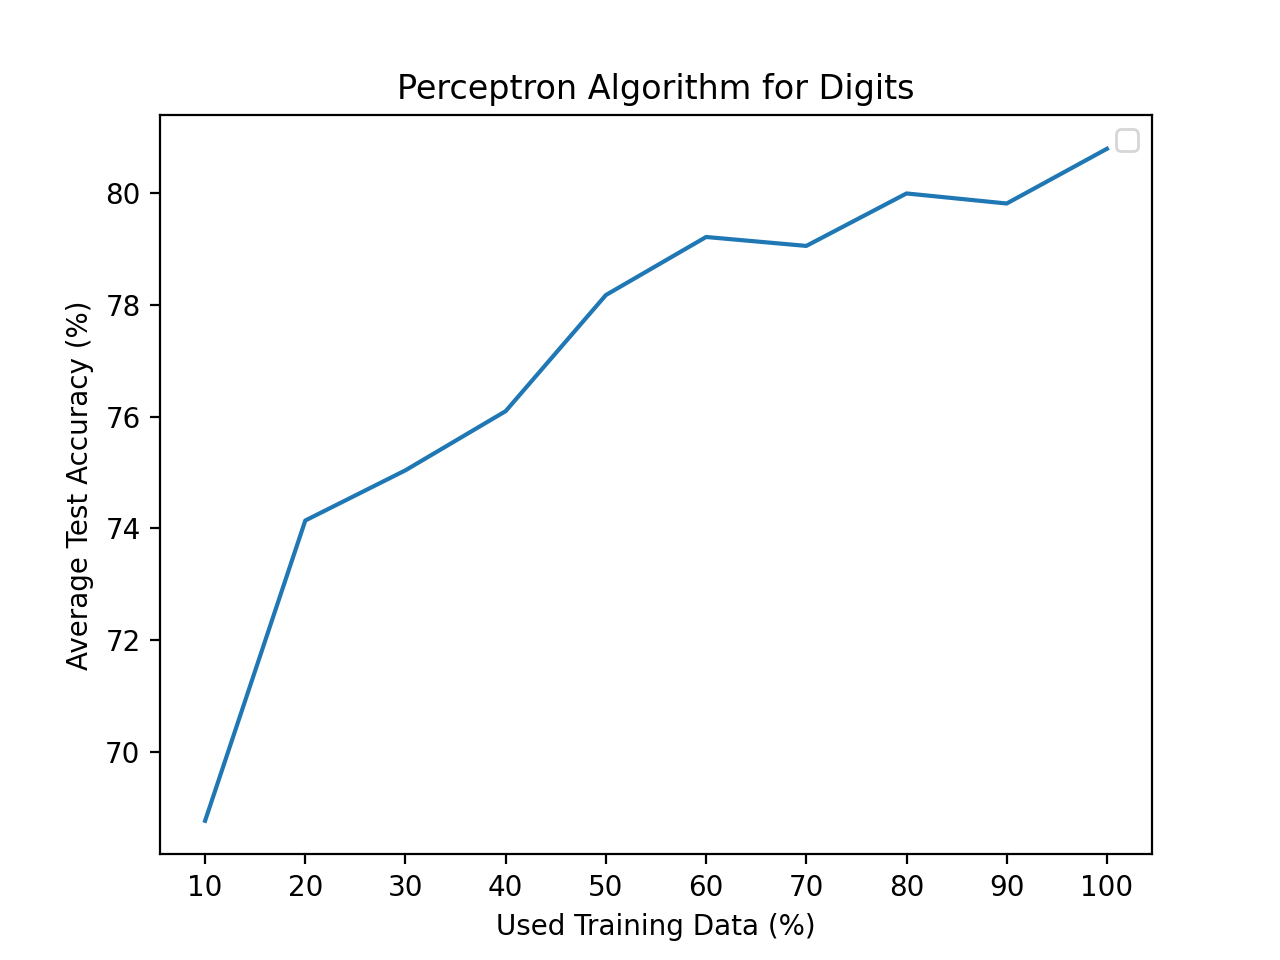
\includegraphics[width=0.8\textwidth]{perDi.png}
        \caption{Average Accuracy of Perceptron for digits}
    \end{figure}
    
    \item Standard deviation plot using Perceptron for digits see Figure 2.
    \begin{figure}
        \centering
        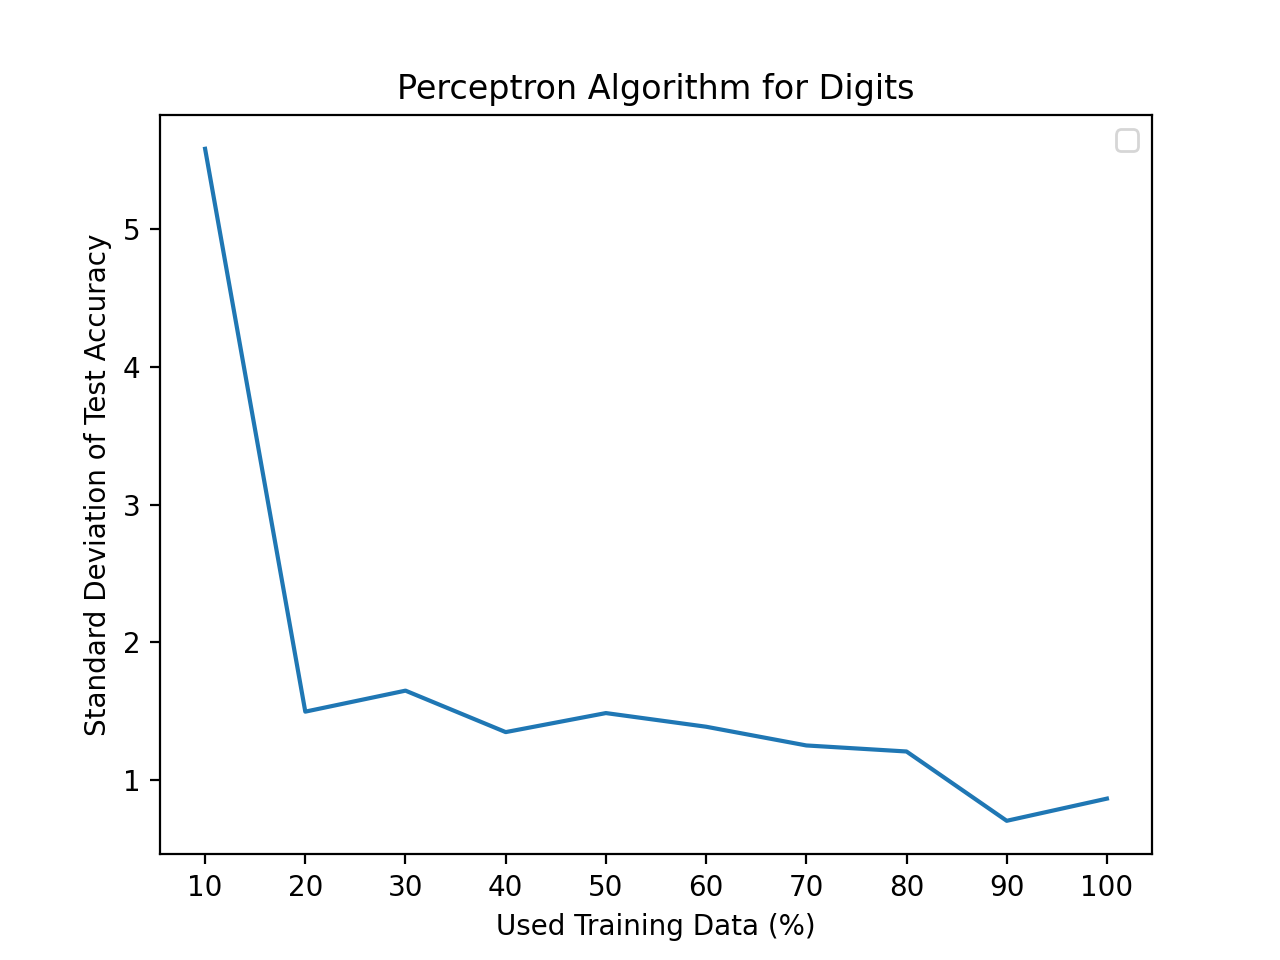
\includegraphics[width=0.8\textwidth]{perDiSd.png}
        \caption{Standard Deviation of Accuracy of Perceptron for digits}
    \end{figure}
    
    \item Time plot using Perceptron for digits see Figure 3.
    \begin{figure}
        \centering
        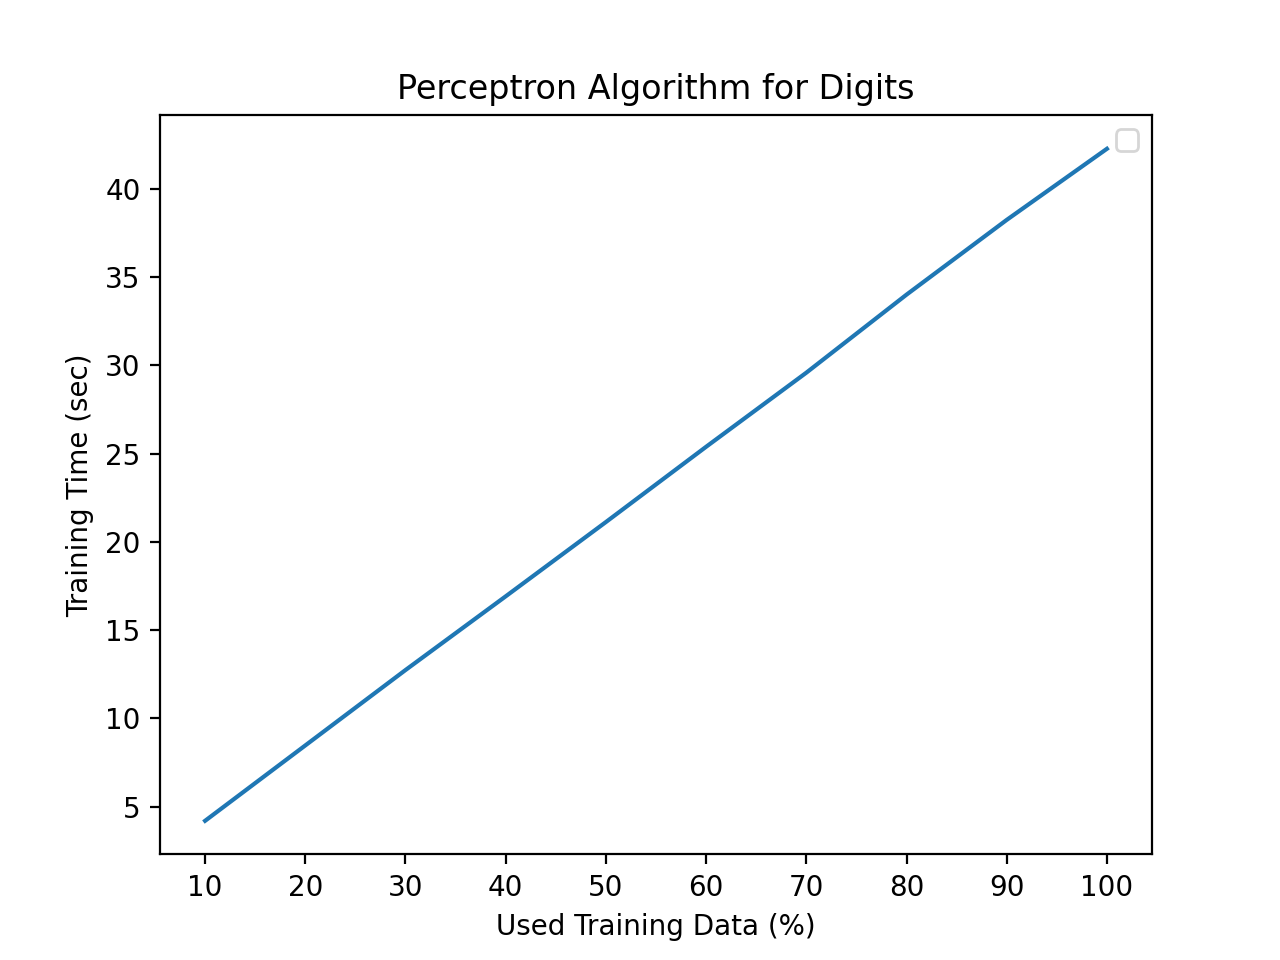
\includegraphics[width=0.8\textwidth]{perDiTime.png}
        \caption{Time of Perceptron for digits}
    \end{figure}
    
    \item Accuracy plot using Perceptron for faces see Figure 4.
    \begin{figure}
        \centering
        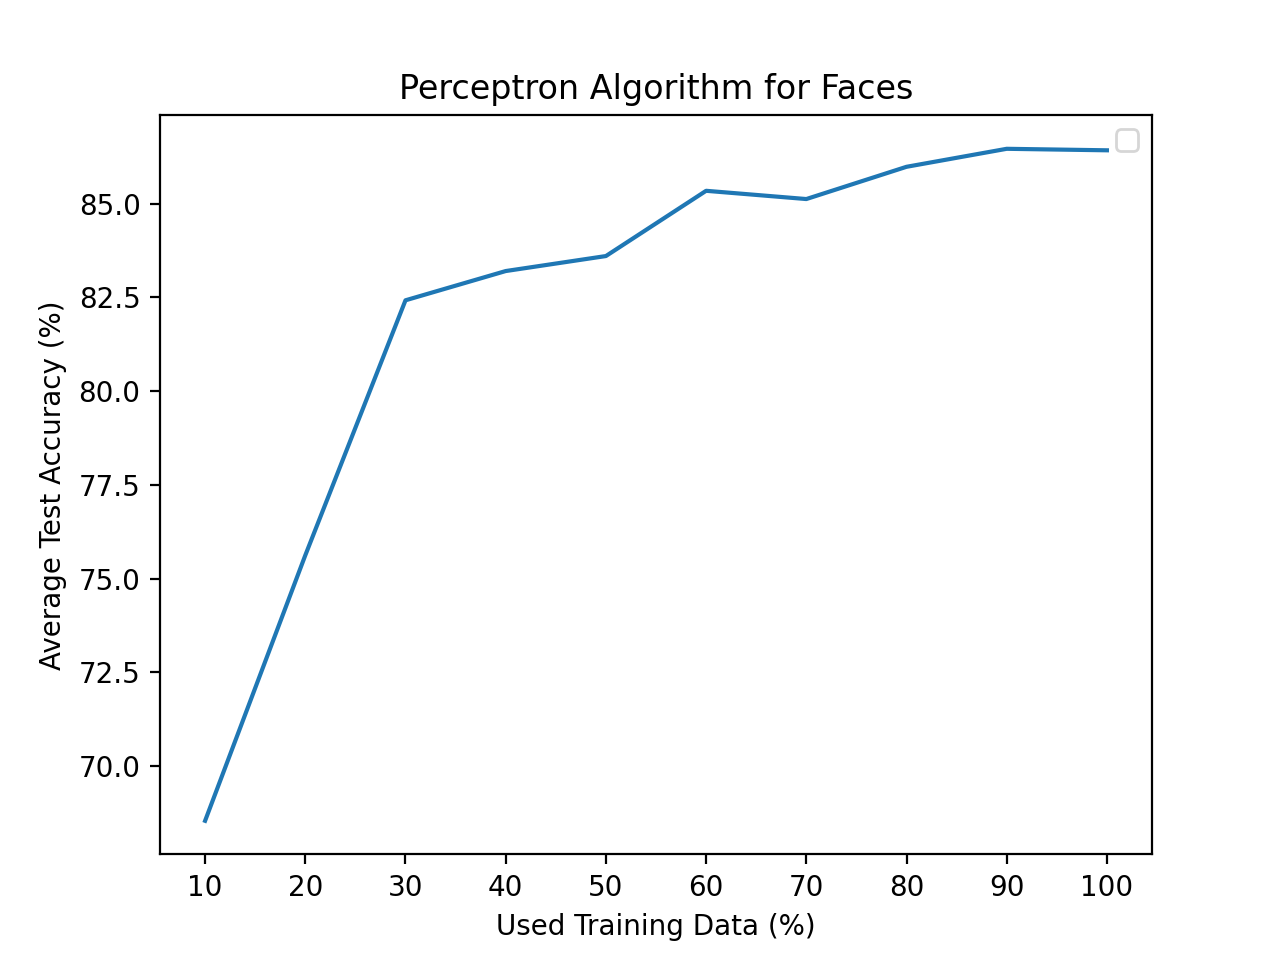
\includegraphics[width=0.8\textwidth]{perFa.png}
        \caption{Average Accuracy of Perceptron for faces}
    \end{figure}
    
    \item Standard deviation plot using Perceptron for faces see Figure 5.
    \begin{figure}
        \centering
        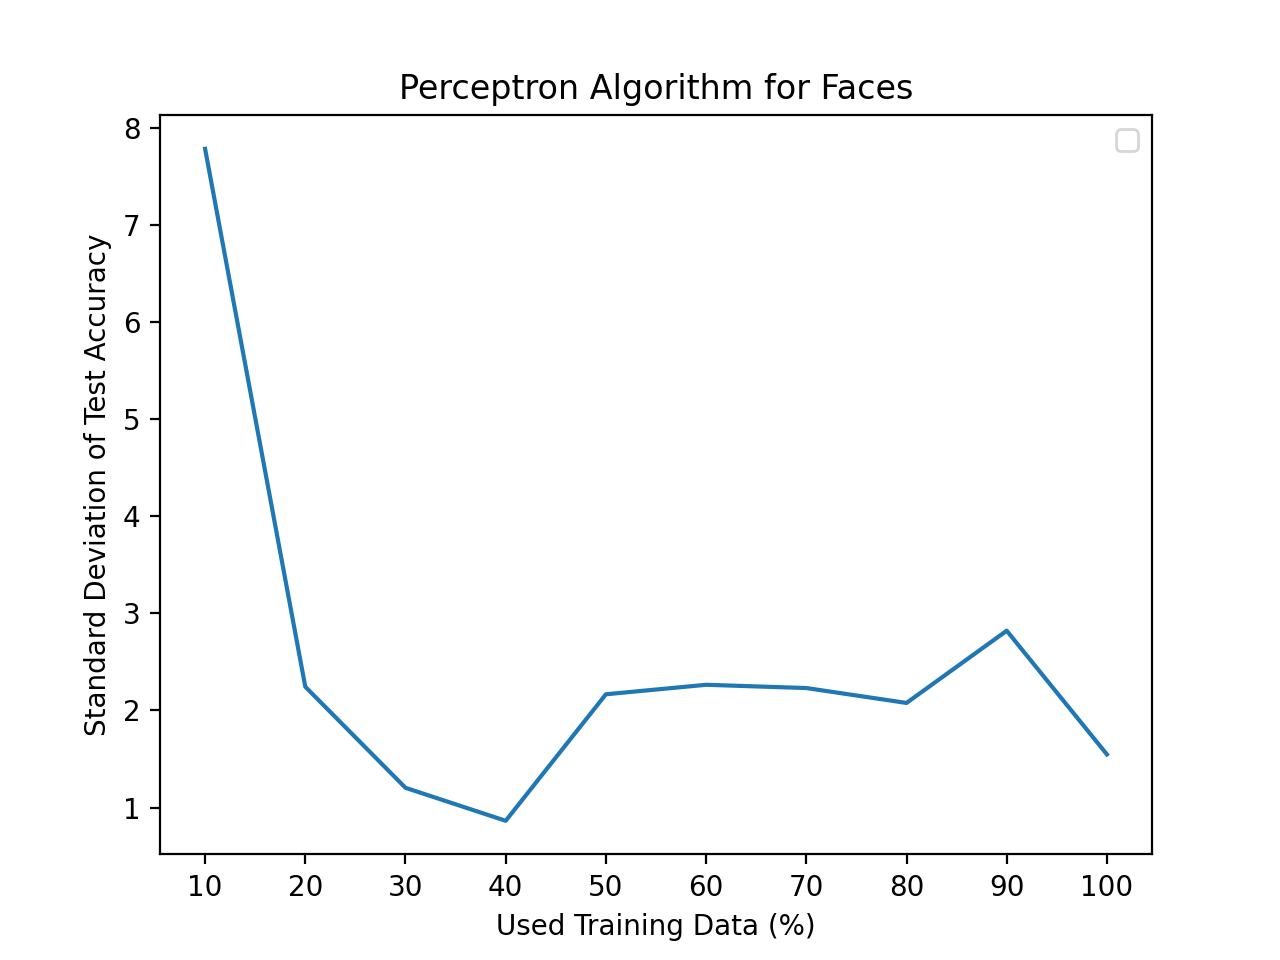
\includegraphics[width=0.8\textwidth]{perFaSd.png}
        \caption{Standard Deviation of Accuracy of Perceptron for faces}
    \end{figure}
    
    \item Time plot using Perceptron for faces see Figure 6.
    \begin{figure}
        \centering
        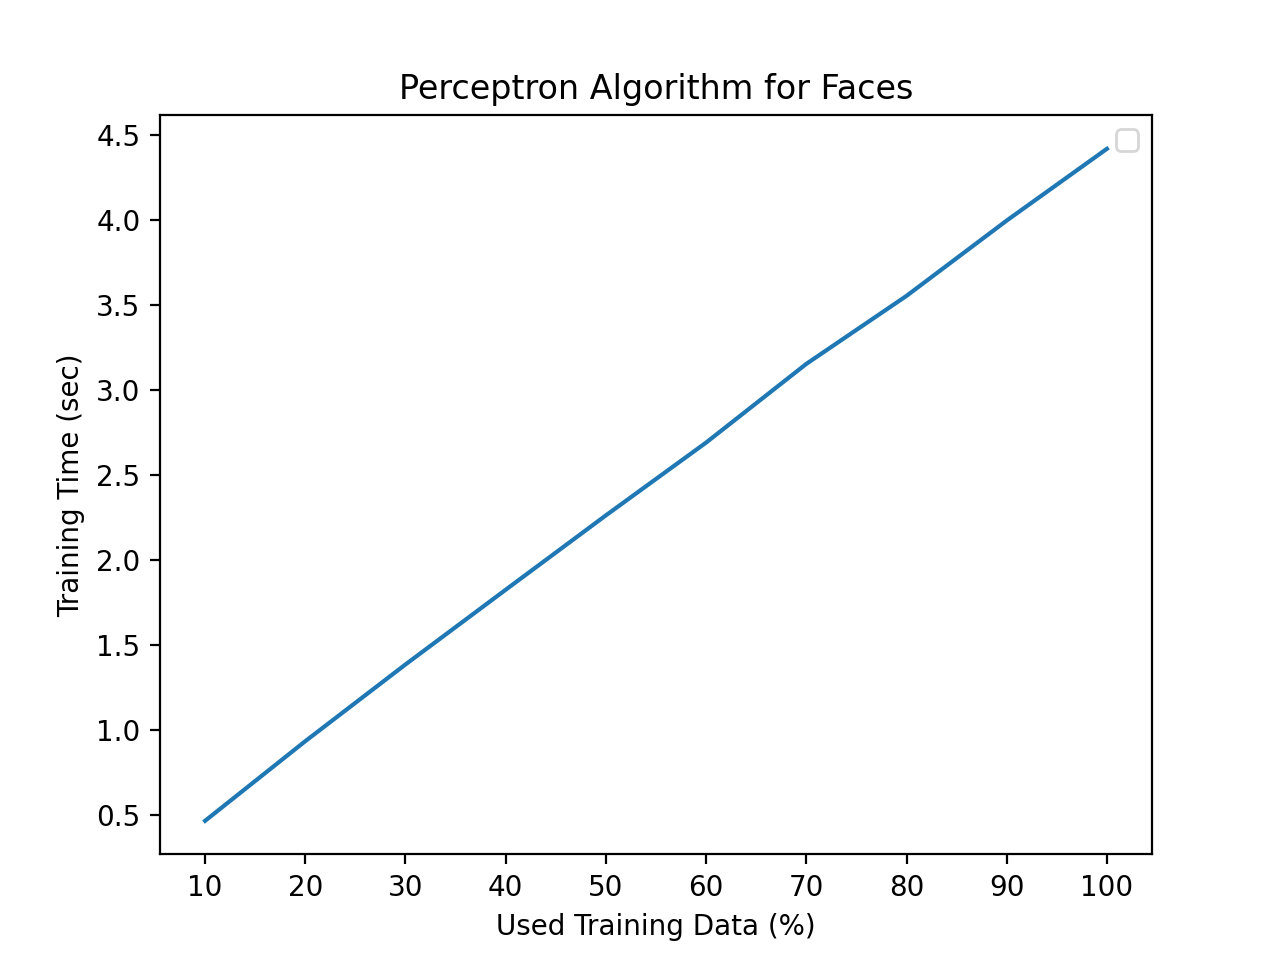
\includegraphics[width=0.8\textwidth]{perFaTime.png}
        \caption{Time of Perceptron for faces}
    \end{figure}
\end{itemize}


\section*{Naive Bayes}
We iterate over all the data and calculate the probability $P(Y=y) = \frac{number of data with label Y = y in training}{total number of training}$. We find the conditional probability for each label, feature, value. For classifying, we take the log of the probability for each label and the label with the max probability is our guess. We train and test the model with $10\%, 20\%, ..., 100\%$ of the training data for both digits and faces.
\begin{itemize}
    \item Accuracy plot using Naive Bayes for digits see Figure 7.
    \begin{figure}
        \centering
        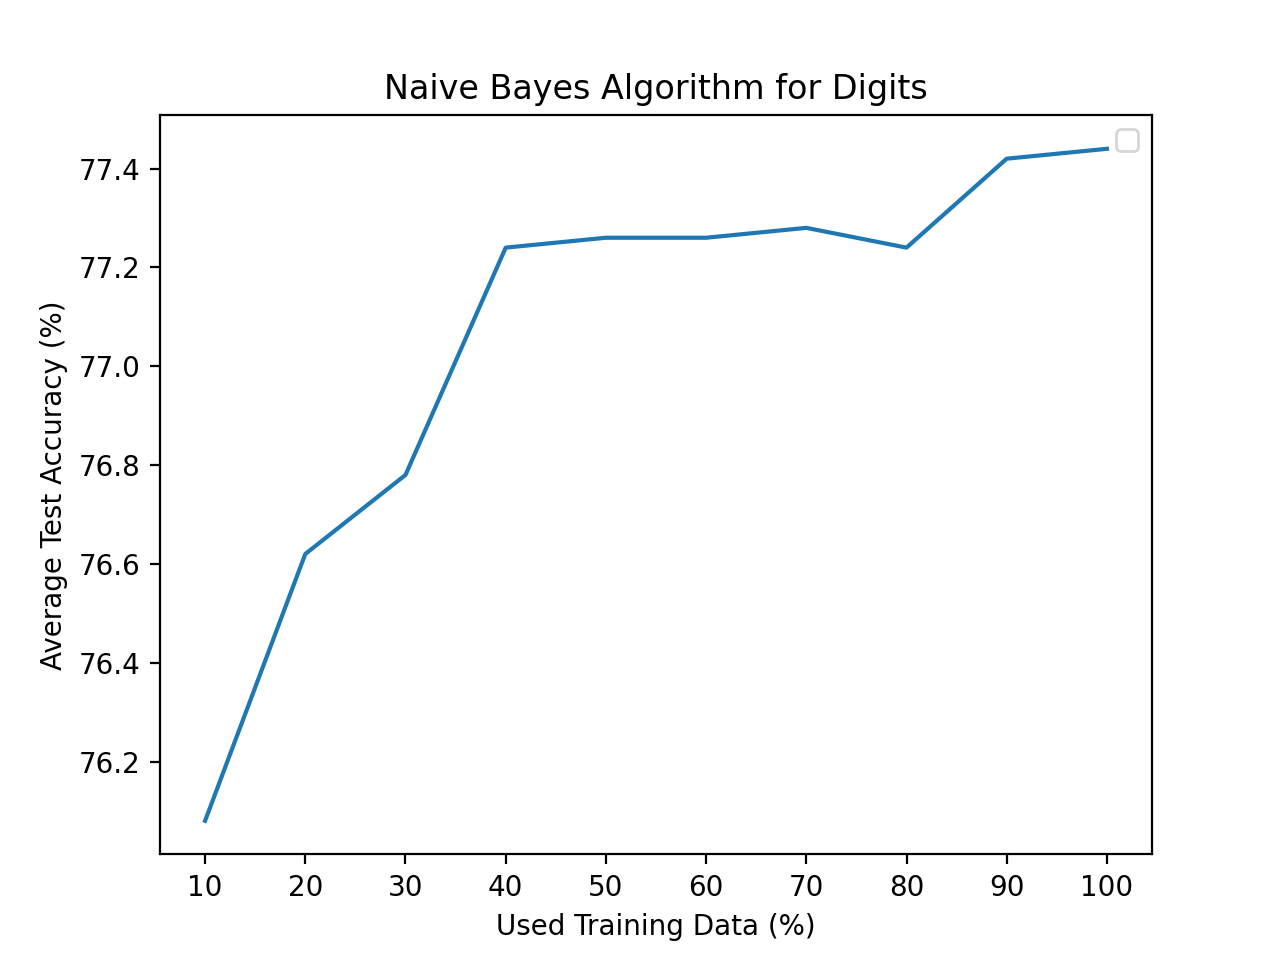
\includegraphics[width=0.8\textwidth]{nbDi.png}
        \caption{Average Accuracy of Naive Bayes for digits}
    \end{figure}
    
    \item Standard deviation plot using Naive Bayes for digits see Figure 8.
    \begin{figure}
        \centering
        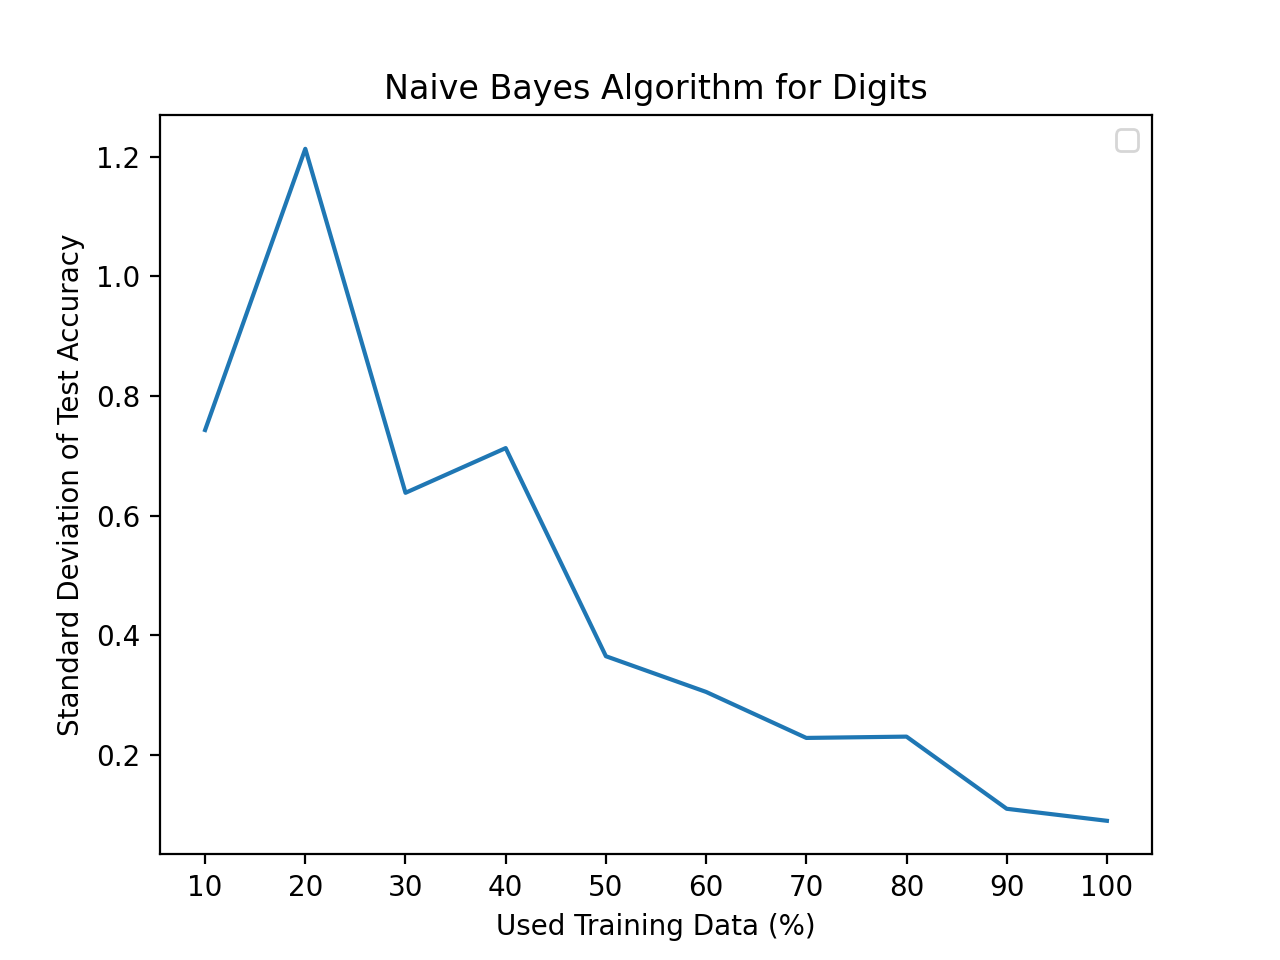
\includegraphics[width=0.8\textwidth]{nbDiSd.png}
        \caption{Standard Deviation of Accuracy of Naive Bayes for digits}
    \end{figure}

    \item Time plot using Naive Bayes for digits see Figure 9.
    \begin{figure}
        \centering
        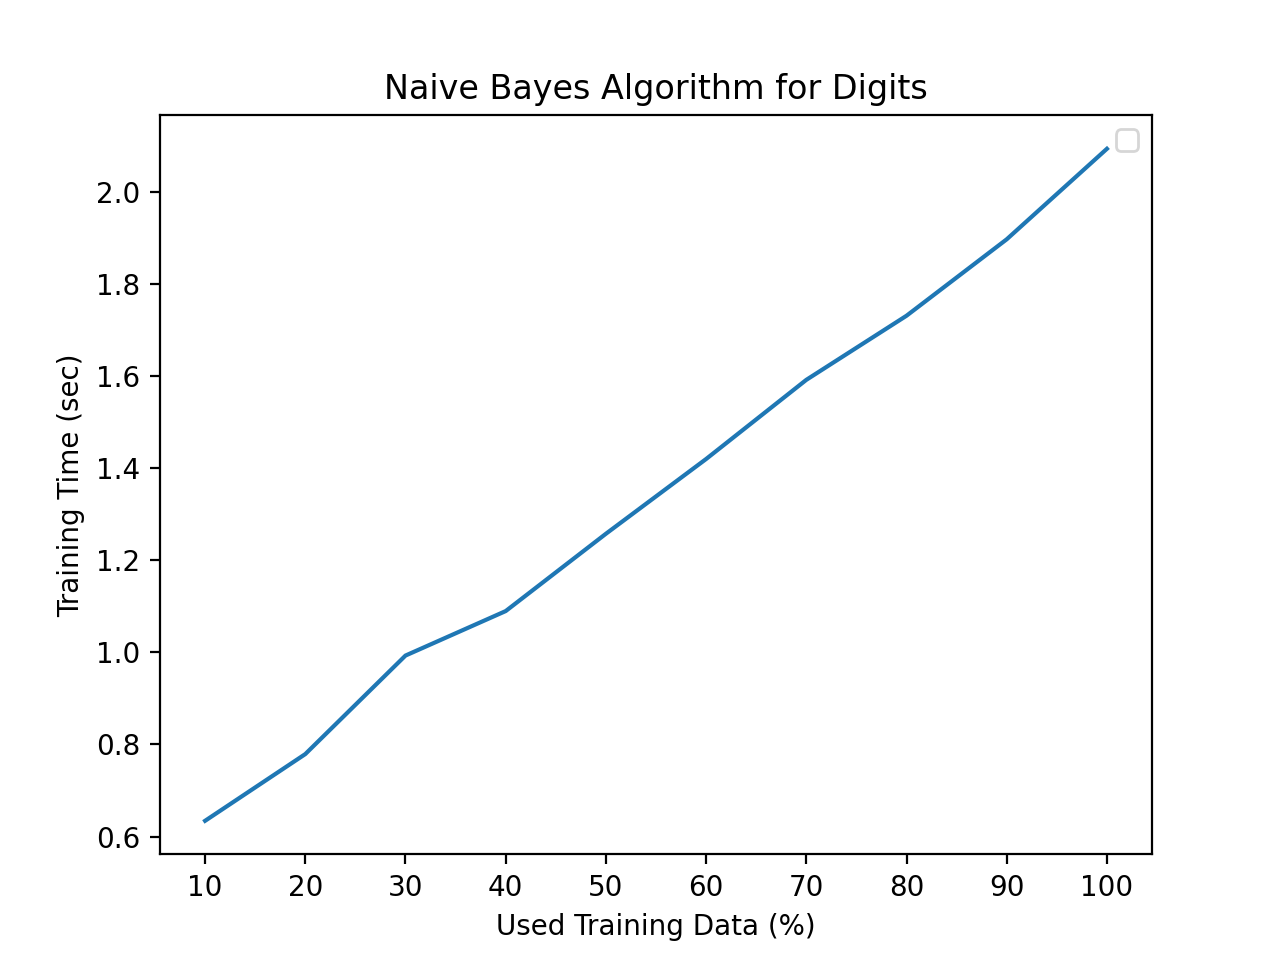
\includegraphics[width=0.8\textwidth]{nbDiTime.png}
        \caption{Time of Naive Bayes for digits}
    \end{figure}
    
    \item Accuracy plot using Naive Bayes for faces see Figure 10.
    \begin{figure}
        \centering
        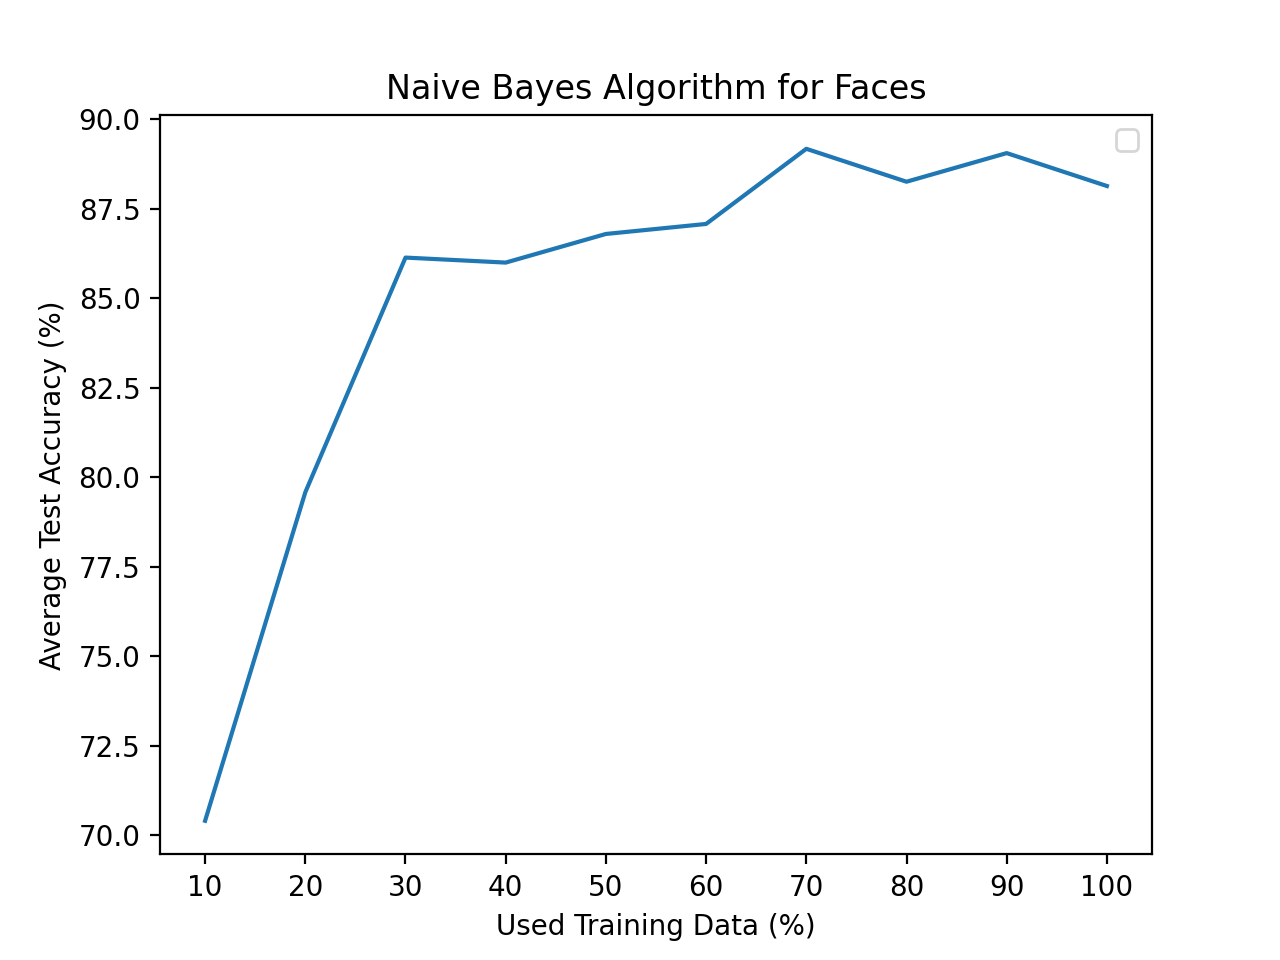
\includegraphics[width=0.8\textwidth]{nbFa.png}
        \caption{Average Accuracy of Naive Bayes for faces}
    \end{figure}
    
    \item Standard deviation plot using Naive Bayes for faces see Figure 11.
    \begin{figure}
        \centering
        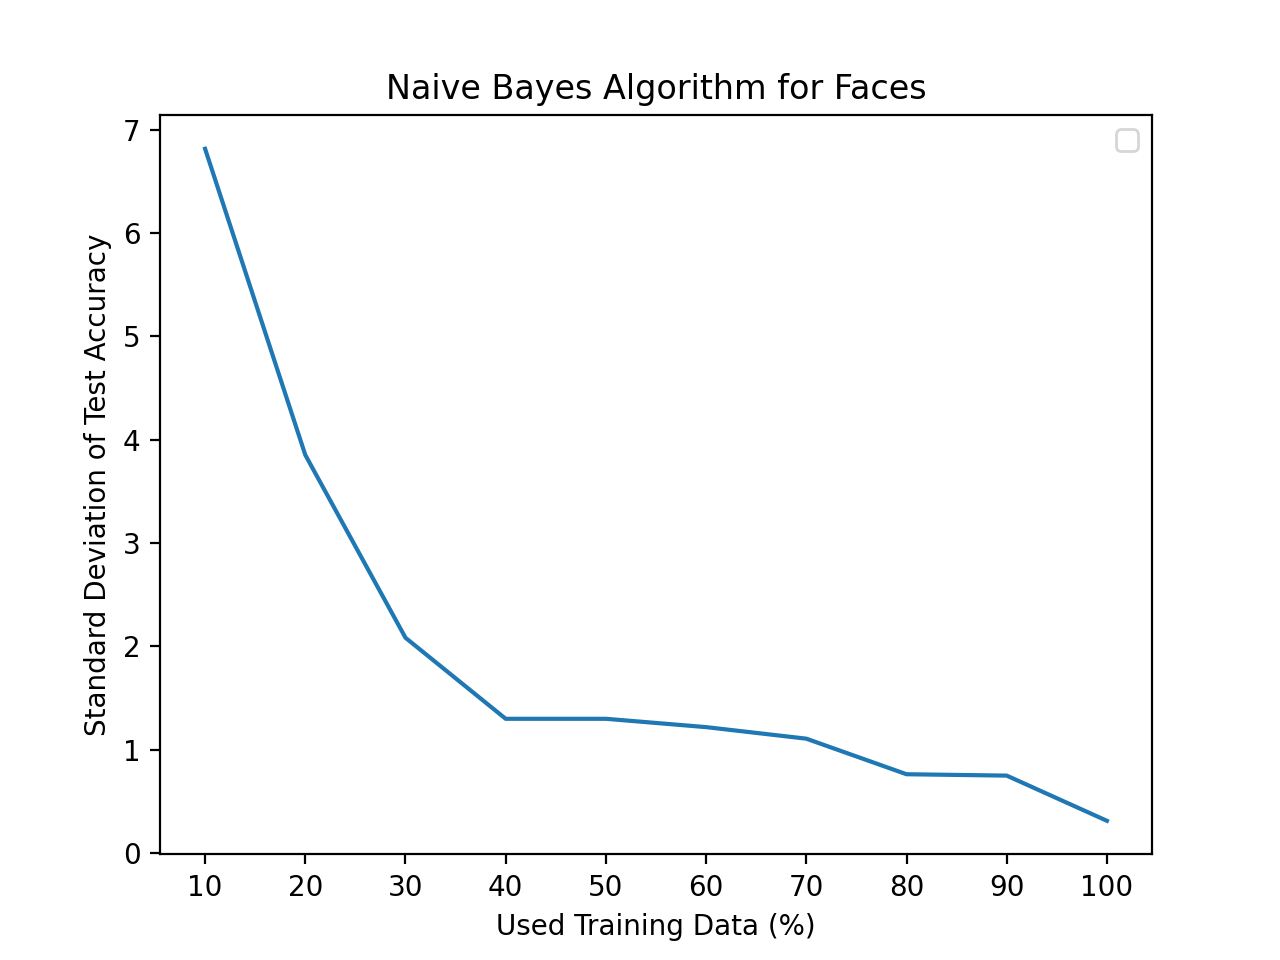
\includegraphics[width=0.8\textwidth]{nbFaSd.png}
        \caption{Standard Deviation of Accuracy of Naive Bayes for faces}
    \end{figure}
    
    \item Time plot using Naive Bayes for faces see Figure 12.
    \begin{figure}
        \centering
        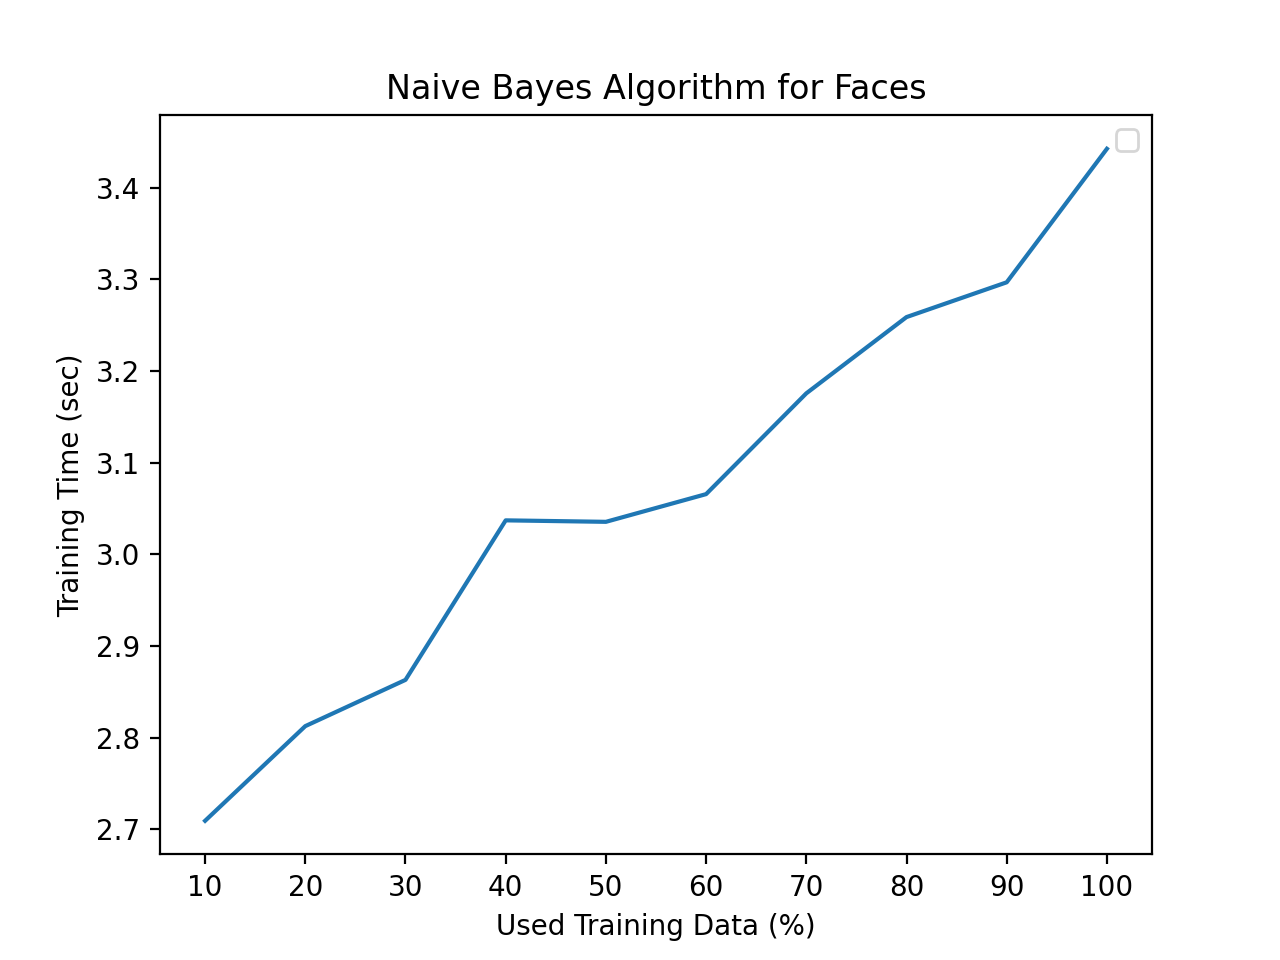
\includegraphics[width=0.8\textwidth]{nbFaTime.png}
        \caption{Time of Naive Bayes for faces}
    \end{figure}
\end{itemize}


\section*{Log Regression}
The logistic regression treat the classification barrier as a linear classifier.  Taking the input data, we first do a normalization on the data and compute the negative log probability for each label. By using stochastic gradient descent, we optimize the average cross-entropy loss batch by batch. For hyperparameter tuning, we try several batch sizes, learning rates and regularization weight and find the best ones. We train and test the model with $10\%, 20\%, ..., 100\%$ of the training data for both digits and faces.
\begin{itemize}
    \item Accuracy plot using Log Regression for digits see Figure 13.
    \begin{figure}
        \centering
        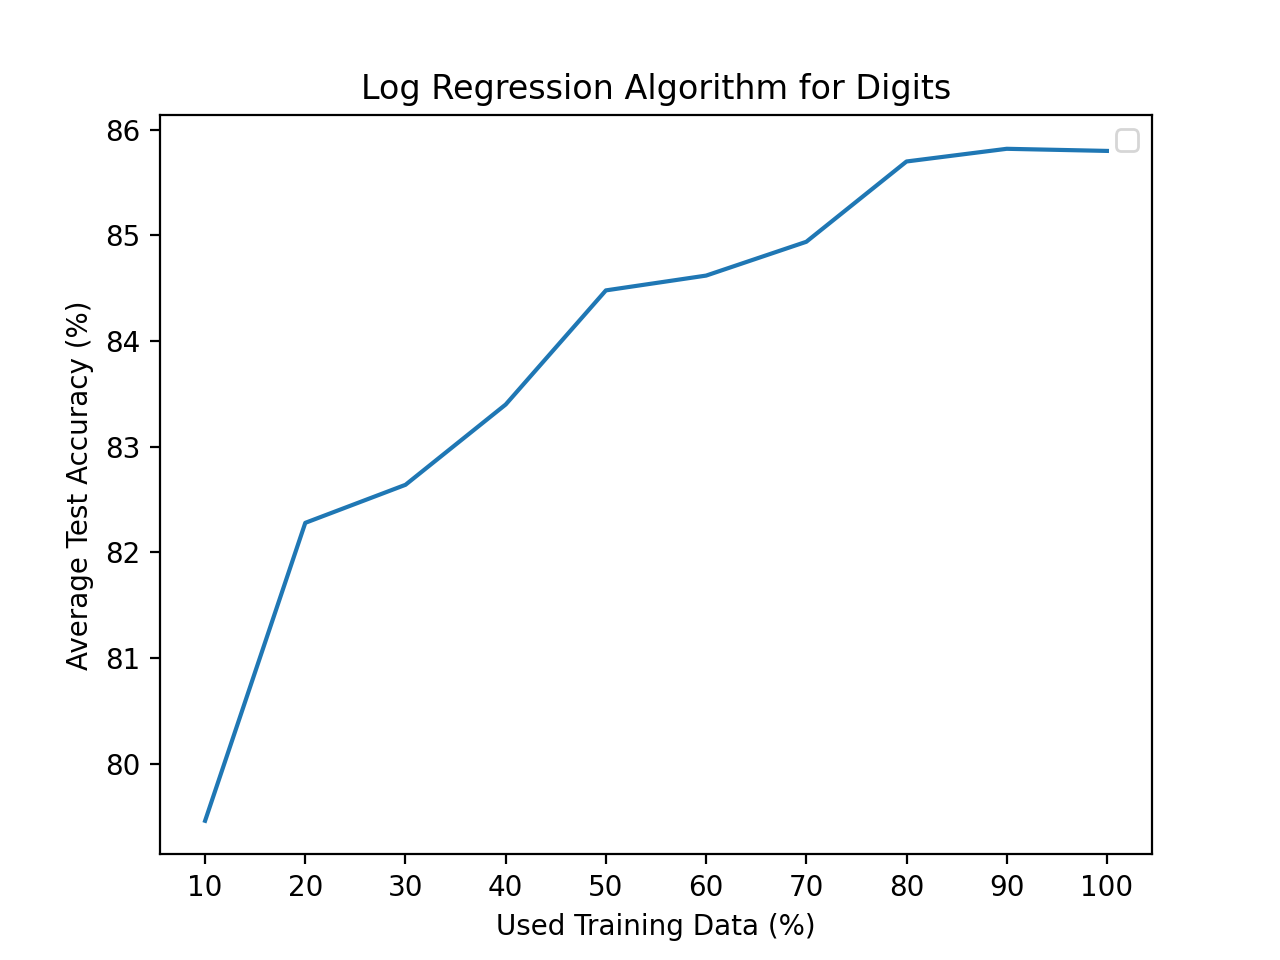
\includegraphics[width=0.8\textwidth]{logDi.png}
        \caption{Average Accuracy of Log Regression for digits}
    \end{figure}
    
    \item Standard deviation plot using Log Regression for digits see Figure 14.
    \begin{figure}
        \centering
        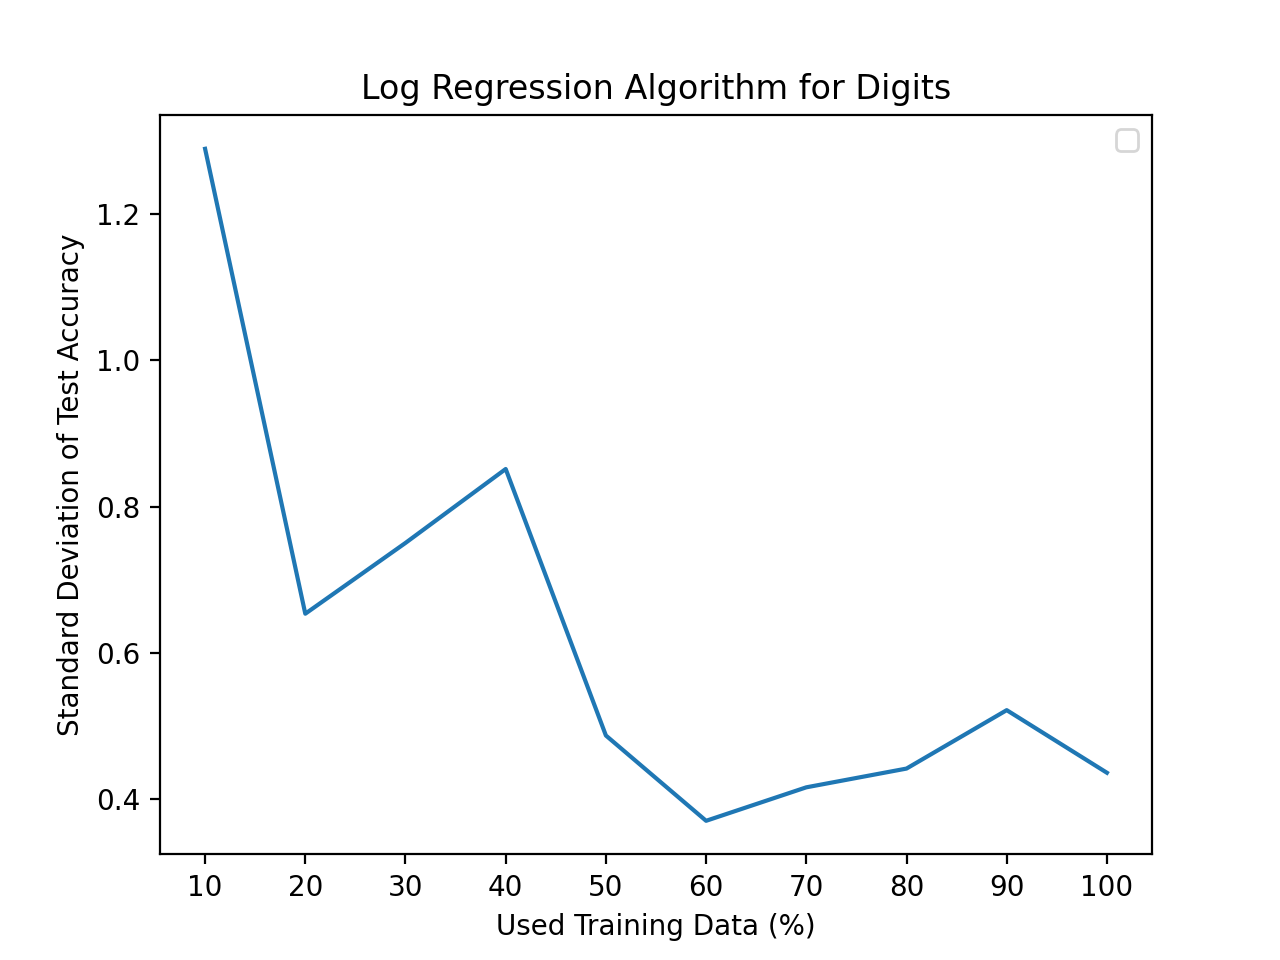
\includegraphics[width=0.8\textwidth]{logDiSd.png}
        \caption{Standard Deviation of Accuracy of Log Regression for digits}
    \end{figure}

    \item Time plot using Log Regression for digits see Figure 15.
    \begin{figure}
        \centering
        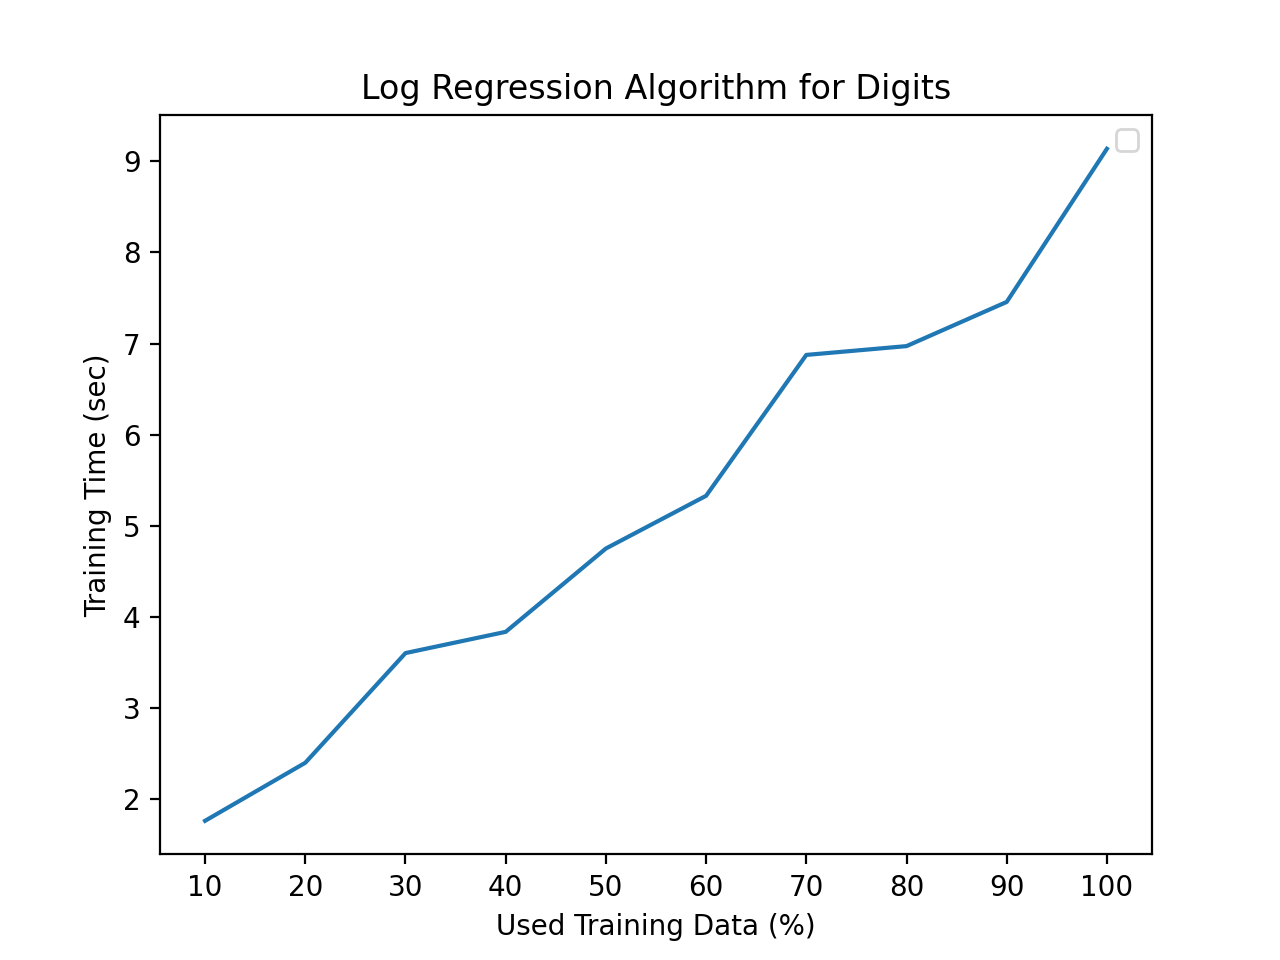
\includegraphics[width=0.8\textwidth]{logDiTime.png}
        \caption{Time of Log Regression for digits}
    \end{figure}
    
    \item Accuracy plot using Log Regression for faces see Figure 16.
    \begin{figure}
        \centering
        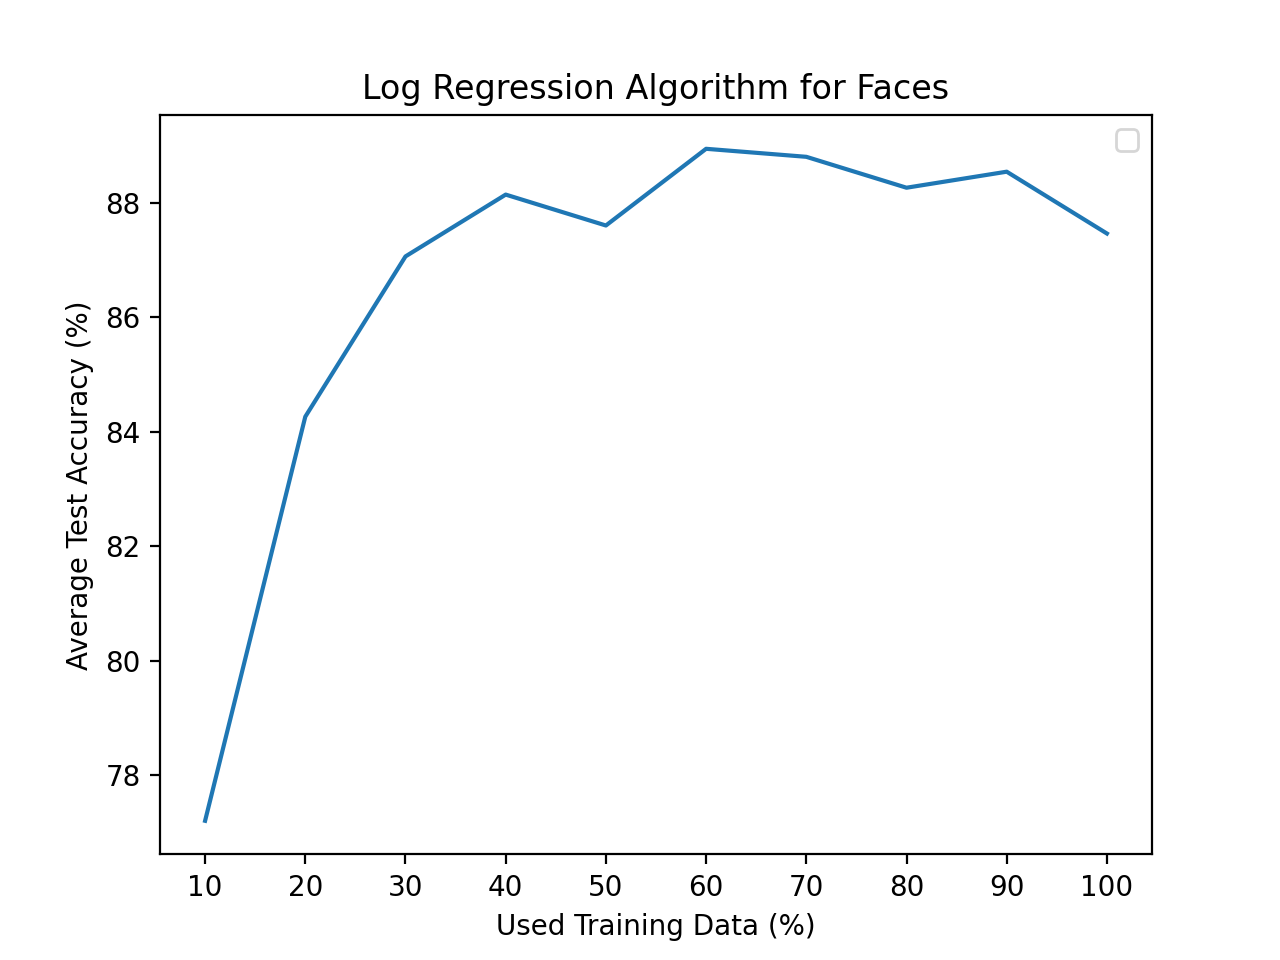
\includegraphics[width=0.8\textwidth]{logFa.png}
        \caption{Average Accuracy of Log Regression for faces}
    \end{figure}
    
    \item Standard deviation plot using Log Regression for faces see Figure 17.
    \begin{figure}
        \centering
        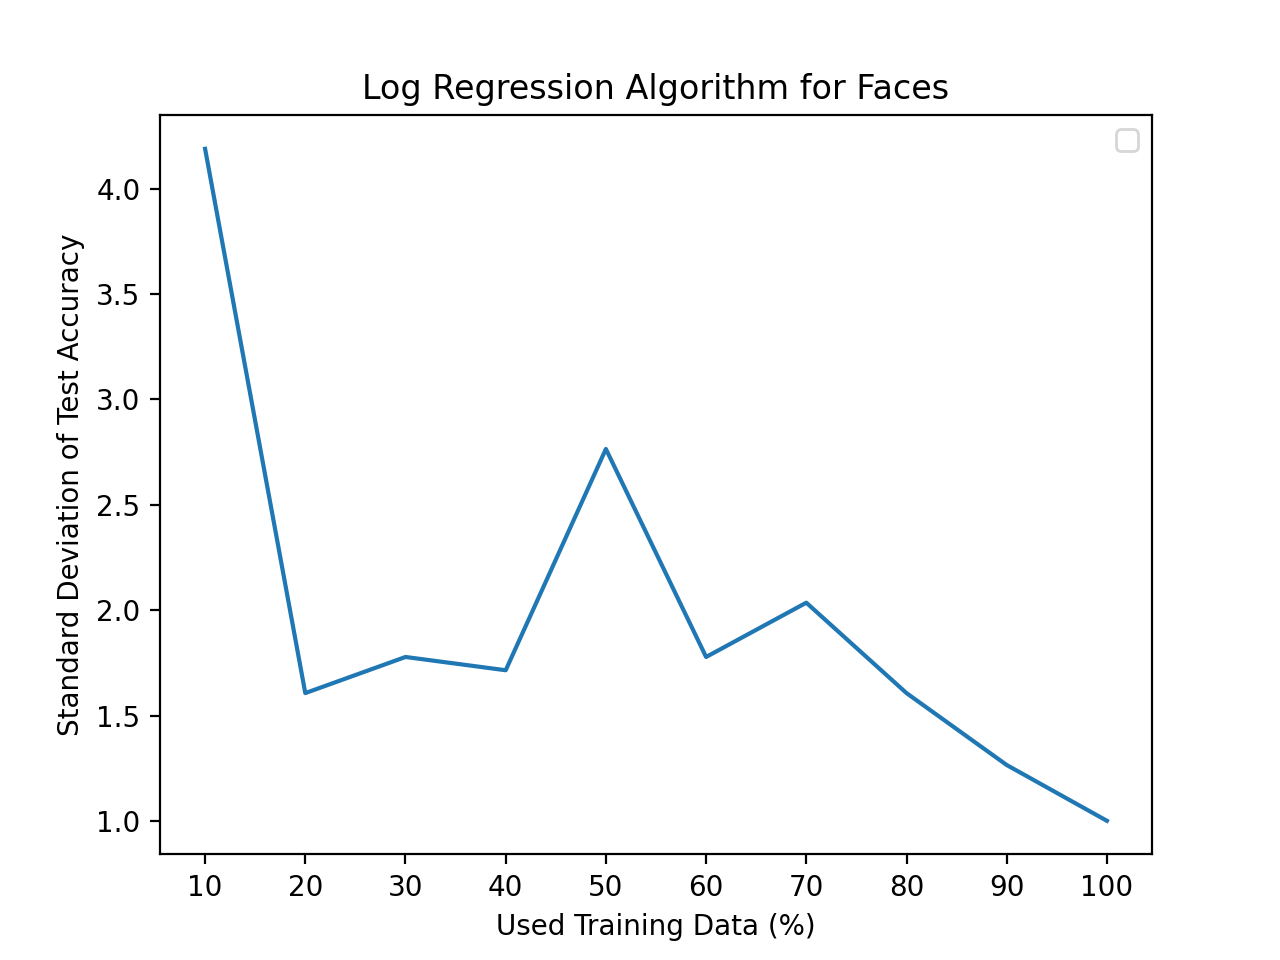
\includegraphics[width=0.8\textwidth]{logFaSd.png}
        \caption{Standard Deviation of Accuracy of Log Regression for faces}
    \end{figure}
    
    \item Time plot using Log Regression for faces see Figure 18.
    \begin{figure}
        \centering
        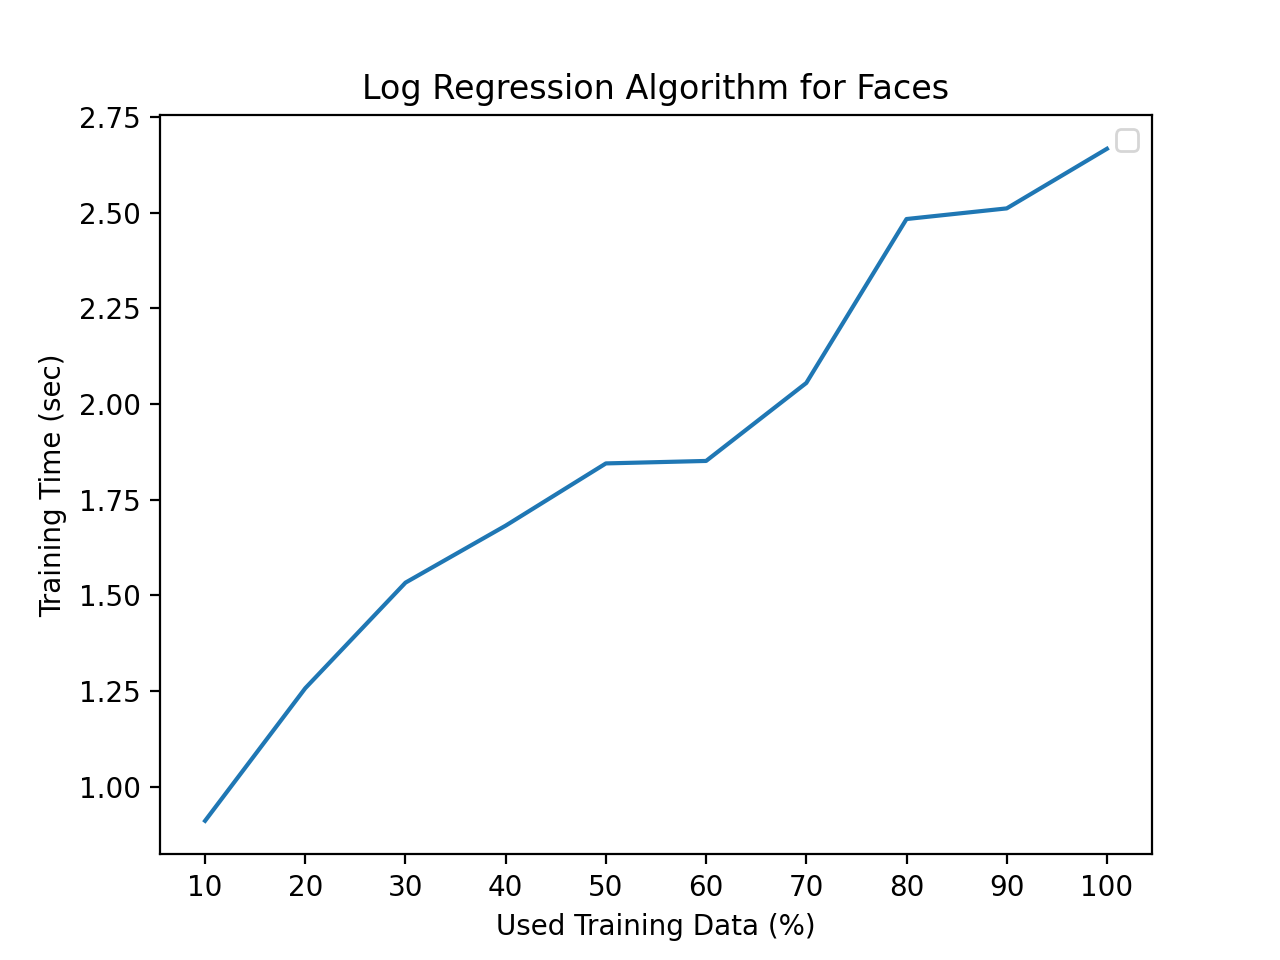
\includegraphics[width=0.8\textwidth]{logFaTime.png}
        \caption{Time of Log Regression for faces}
    \end{figure}
\end{itemize}

\end{document}